\documentclass{standalone}
\usepackage{tikz}
\usetikzlibrary{patterns, positioning}


\begin{document}
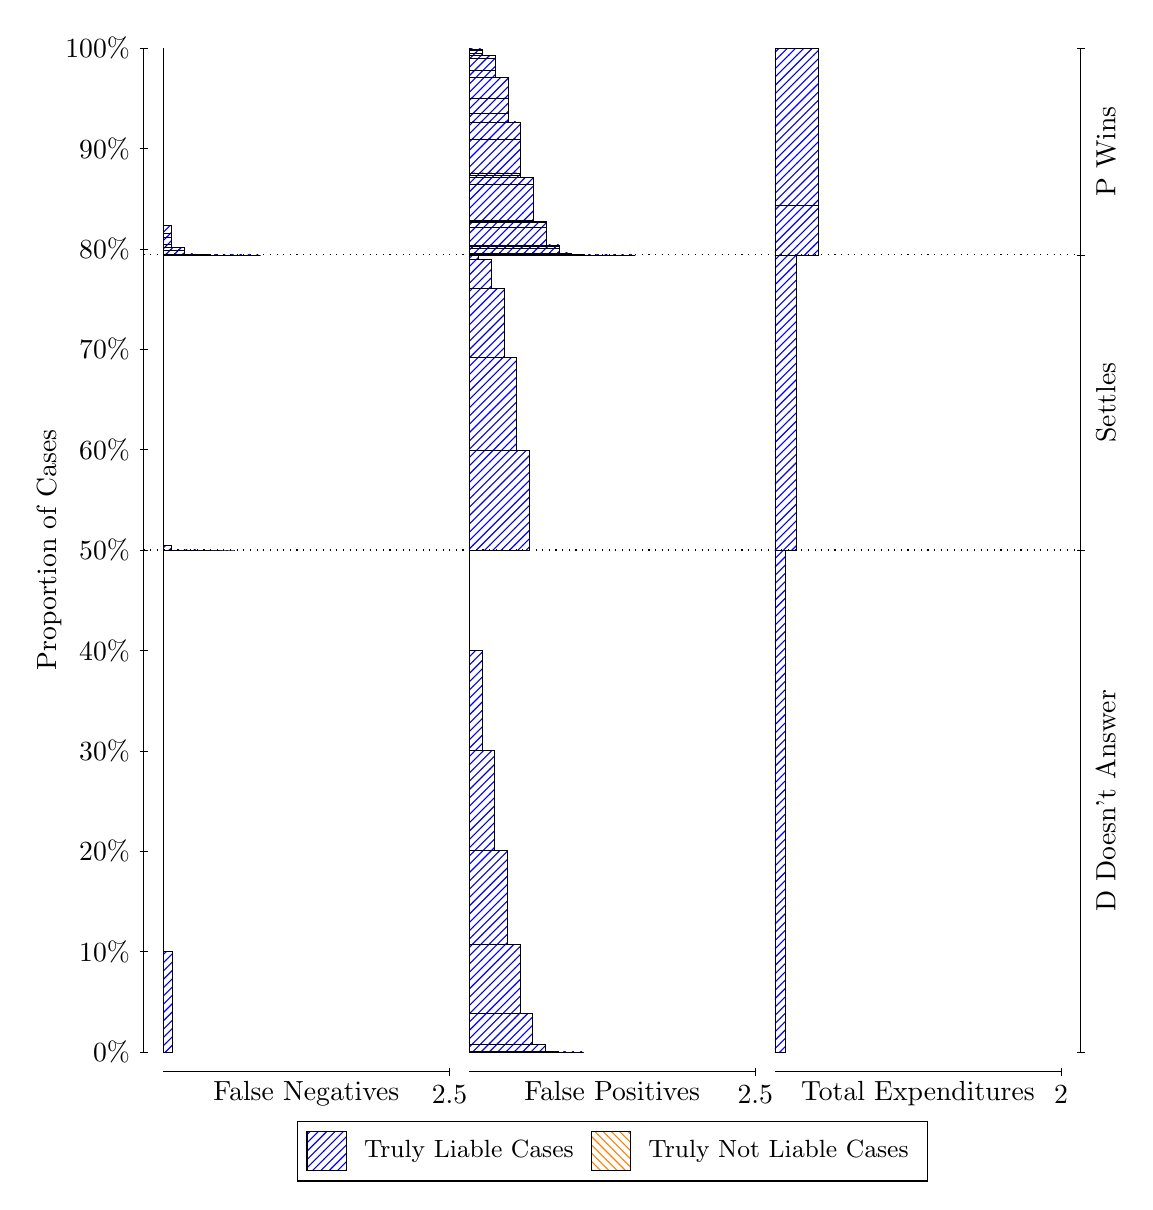
\begin{tikzpicture}
\draw[black, very thin] (1.5,1.75) -- (1.5,14.5);
\node[rotate=90, text=black, anchor=center] at (0.3, 8.125) {Proportion of Cases};
\draw[black, very thin] (1.45,1.75) -- (1.55,1.75);
\node[text=black, anchor=east] at (1.45, 1.75) {0\%};
\draw[black, very thin] (1.45,3.025) -- (1.55,3.025);
\node[text=black, anchor=east] at (1.45, 3.025) {10\%};
\draw[black, very thin] (1.45,4.3) -- (1.55,4.3);
\node[text=black, anchor=east] at (1.45, 4.3) {20\%};
\draw[black, very thin] (1.45,5.575) -- (1.55,5.575);
\node[text=black, anchor=east] at (1.45, 5.575) {30\%};
\draw[black, very thin] (1.45,6.85) -- (1.55,6.85);
\node[text=black, anchor=east] at (1.45, 6.85) {40\%};
\draw[black, very thin] (1.45,8.125) -- (1.55,8.125);
\node[text=black, anchor=east] at (1.45, 8.125) {50\%};
\draw[black, very thin] (1.45,9.4) -- (1.55,9.4);
\node[text=black, anchor=east] at (1.45, 9.4) {60\%};
\draw[black, very thin] (1.45,10.675) -- (1.55,10.675);
\node[text=black, anchor=east] at (1.45, 10.675) {70\%};
\draw[black, very thin] (1.45,11.95) -- (1.55,11.95);
\node[text=black, anchor=east] at (1.45, 11.95) {80\%};
\draw[black, very thin] (1.45,13.225) -- (1.55,13.225);
\node[text=black, anchor=east] at (1.45, 13.225) {90\%};
\draw[black, very thin] (1.45,14.5) -- (1.55,14.5);
\node[text=black, anchor=east] at (1.45, 14.5) {100\%};

\draw[black, very thin] (13.4,1.75) -- (13.4,14.5);
\draw[black, very thin] (13.35,1.75) -- (13.45,1.75);
\node[anchor=west] at (13.35, 1.75) {};
\draw[black, very thin] (13.35,8.125) -- (13.45,8.125);
\node[anchor=west] at (13.35, 8.125) {};
\draw[black, very thin] (13.35,11.874) -- (13.45,11.874);
\node[anchor=west] at (13.35, 11.874) {};
\draw[black, very thin] (13.35,14.5) -- (13.45,14.5);
\node[anchor=west] at (13.35, 14.5) {};

\draw[black, very thin, pattern color=blue, pattern=north east lines] (1.75,1.75) rectangle (1.859,3.025);
\draw[black, very thin, pattern color=orange, pattern=north west lines] (1.75,3.025) rectangle (1.75,3.025);
\draw[black, very thin, pattern color=blue, pattern=north east lines] (1.75,3.025) rectangle (1.75,8.125);
\draw[black, very thin, pattern color=blue, pattern=north east lines] (1.75,8.125) rectangle (2.6583,8.125);
\draw[black, very thin, pattern color=blue, pattern=north east lines] (1.75,8.125) rectangle (2.4969,8.125);
\draw[black, very thin, pattern color=blue, pattern=north east lines] (1.75,8.125) rectangle (2.3354,8.125);
\draw[black, very thin, pattern color=blue, pattern=north east lines] (1.75,8.125) rectangle (2.1739,8.1251);
\draw[black, very thin, pattern color=blue, pattern=north east lines] (1.75,8.1251) rectangle (2.0124,8.1275);
\draw[black, very thin, pattern color=blue, pattern=north east lines] (1.75,8.1275) rectangle (1.8509,8.1864);
\draw[black, very thin, pattern color=orange, pattern=north west lines] (1.75,8.1864) rectangle (1.75,8.1864);
\draw[black, very thin, pattern color=blue, pattern=north east lines] (1.75,8.1864) rectangle (1.75,11.874);
\draw[black, very thin, pattern color=blue, pattern=north east lines] (1.75,11.874) rectangle (2.9853,11.874);
\draw[black, very thin, pattern color=blue, pattern=north east lines] (1.75,11.874) rectangle (2.8239,11.874);
\draw[black, very thin, pattern color=blue, pattern=north east lines] (1.75,11.874) rectangle (2.8239,11.874);
\draw[black, very thin, pattern color=blue, pattern=north east lines] (1.75,11.874) rectangle (2.6624,11.874);
\draw[black, very thin, pattern color=blue, pattern=north east lines] (1.75,11.874) rectangle (2.5009,11.874);
\draw[black, very thin, pattern color=blue, pattern=north east lines] (1.75,11.874) rectangle (2.5009,11.874);
\draw[black, very thin, pattern color=blue, pattern=north east lines] (1.75,11.874) rectangle (2.3394,11.875);
\draw[black, very thin, pattern color=blue, pattern=north east lines] (1.75,11.875) rectangle (2.1779,11.878);
\draw[black, very thin, pattern color=blue, pattern=north east lines] (1.75,11.878) rectangle (2.1779,11.886);
\draw[black, very thin, pattern color=blue, pattern=north east lines] (1.75,11.886) rectangle (2.0164,11.935);
\draw[black, very thin, pattern color=blue, pattern=north east lines] (1.75,11.935) rectangle (2.0164,11.967);
\draw[black, very thin, pattern color=blue, pattern=north east lines] (1.75,11.967) rectangle (2.0164,11.967);
\draw[black, very thin, pattern color=blue, pattern=north east lines] (1.75,11.967) rectangle (1.855,12.01);
\draw[black, very thin, pattern color=blue, pattern=north east lines] (1.75,12.01) rectangle (1.855,12.102);
\draw[black, very thin, pattern color=blue, pattern=north east lines] (1.75,12.102) rectangle (1.855,12.148);
\draw[black, very thin, pattern color=blue, pattern=north east lines] (1.75,12.148) rectangle (1.855,12.25);
\draw[black, very thin, pattern color=orange, pattern=north west lines] (1.75,12.25) rectangle (1.75,12.25);
\draw[black, very thin, pattern color=blue, pattern=north east lines] (1.75,12.25) rectangle (1.75,14.5);
\draw[black, very thin, pattern color=orange, pattern=north west lines] (5.6333,1.75) rectangle (7.0867,1.75);
\draw[black, very thin, pattern color=blue, pattern=north east lines] (5.6333,1.75) rectangle (7.0867,1.75);
\draw[black, very thin, pattern color=blue, pattern=north east lines] (5.6333,1.75) rectangle (6.9252,1.7503);
\draw[black, very thin, pattern color=blue, pattern=north east lines] (5.6333,1.7503) rectangle (6.7637,1.7583);
\draw[black, very thin, pattern color=blue, pattern=north east lines] (5.6333,1.7583) rectangle (6.6022,1.8435);
\draw[black, very thin, pattern color=blue, pattern=north east lines] (5.6333,1.8435) rectangle (6.4407,2.2369);
\draw[black, very thin, pattern color=blue, pattern=north east lines] (5.6333,2.2369) rectangle (6.2793,3.1185);
\draw[black, very thin, pattern color=blue, pattern=north east lines] (5.6333,3.1185) rectangle (6.1178,4.3083);
\draw[black, very thin, pattern color=blue, pattern=north east lines] (5.6333,4.3083) rectangle (5.9563,5.5753);
\draw[black, very thin, pattern color=blue, pattern=north east lines] (5.6333,5.5753) rectangle (5.7948,6.85);
\draw[black, very thin, pattern color=blue, pattern=north east lines] (5.6333,6.85) rectangle (5.6333,8.125);
\draw[black, very thin, pattern color=orange, pattern=north west lines] (5.6333,8.125) rectangle (6.3963,8.125);
\draw[black, very thin, pattern color=blue, pattern=north east lines] (5.6333,8.125) rectangle (6.3963,9.3886);
\draw[black, very thin, pattern color=blue, pattern=north east lines] (5.6333,9.3886) rectangle (6.2349,10.572);
\draw[black, very thin, pattern color=blue, pattern=north east lines] (5.6333,10.572) rectangle (6.0734,11.446);
\draw[black, very thin, pattern color=blue, pattern=north east lines] (5.6333,11.446) rectangle (5.9119,11.813);
\draw[black, very thin, pattern color=blue, pattern=north east lines] (5.6333,11.813) rectangle (5.7504,11.871);
\draw[black, very thin, pattern color=blue, pattern=north east lines] (5.6333,11.871) rectangle (5.6333,11.874);
\draw[black, very thin, pattern color=orange, pattern=north west lines] (5.6333,11.874) rectangle (7.7407,11.874);
\draw[black, very thin, pattern color=blue, pattern=north east lines] (5.6333,11.874) rectangle (7.7407,11.874);
\draw[black, very thin, pattern color=orange, pattern=north west lines] (5.6333,11.874) rectangle (7.5792,11.874);
\draw[black, very thin, pattern color=blue, pattern=north east lines] (5.6333,11.874) rectangle (7.5792,11.874);
\draw[black, very thin, pattern color=orange, pattern=north west lines] (5.6333,11.874) rectangle (7.4177,11.874);
\draw[black, very thin, pattern color=blue, pattern=north east lines] (5.6333,11.874) rectangle (7.4177,11.874);
\draw[black, very thin, pattern color=blue, pattern=north east lines] (5.6333,11.874) rectangle (7.4177,11.874);
\draw[black, very thin, pattern color=orange, pattern=north west lines] (5.6333,11.874) rectangle (7.2562,11.874);
\draw[black, very thin, pattern color=blue, pattern=north east lines] (5.6333,11.874) rectangle (7.2562,11.874);
\draw[black, very thin, pattern color=orange, pattern=north west lines] (5.6333,11.874) rectangle (7.0947,11.874);
\draw[black, very thin, pattern color=blue, pattern=north east lines] (5.6333,11.874) rectangle (7.0947,11.877);
\draw[black, very thin, pattern color=blue, pattern=north east lines] (5.6333,11.877) rectangle (6.9333,11.884);
\draw[black, very thin, pattern color=blue, pattern=north east lines] (5.6333,11.884) rectangle (6.9333,11.887);
\draw[black, very thin, pattern color=orange, pattern=north west lines] (5.6333,11.887) rectangle (6.9333,11.887);
\draw[black, very thin, pattern color=blue, pattern=north east lines] (5.6333,11.887) rectangle (6.9333,11.899);
\draw[black, very thin, pattern color=blue, pattern=north east lines] (5.6333,11.899) rectangle (6.7718,11.962);
\draw[black, very thin, pattern color=blue, pattern=north east lines] (5.6333,11.962) rectangle (6.7718,11.98);
\draw[black, very thin, pattern color=orange, pattern=north west lines] (5.6333,11.98) rectangle (6.7718,11.98);
\draw[black, very thin, pattern color=blue, pattern=north east lines] (5.6333,11.98) rectangle (6.7718,12);
\draw[black, very thin, pattern color=blue, pattern=north east lines] (5.6333,12) rectangle (6.6103,12.227);
\draw[black, very thin, pattern color=orange, pattern=north west lines] (5.6333,12.227) rectangle (6.6103,12.227);
\draw[black, very thin, pattern color=blue, pattern=north east lines] (5.6333,12.227) rectangle (6.6103,12.285);
\draw[black, very thin, pattern color=blue, pattern=north east lines] (5.6333,12.285) rectangle (6.6103,12.297);
\draw[black, very thin, pattern color=blue, pattern=north east lines] (5.6333,12.297) rectangle (6.4488,12.315);
\draw[black, very thin, pattern color=orange, pattern=north west lines] (5.6333,12.315) rectangle (6.4488,12.315);
\draw[black, very thin, pattern color=blue, pattern=north east lines] (5.6333,12.315) rectangle (6.4488,12.774);
\draw[black, very thin, pattern color=blue, pattern=north east lines] (5.6333,12.774) rectangle (6.4488,12.862);
\draw[black, very thin, pattern color=blue, pattern=north east lines] (5.6333,12.862) rectangle (6.2873,12.887);
\draw[black, very thin, pattern color=blue, pattern=north east lines] (5.6333,12.887) rectangle (6.2873,12.915);
\draw[black, very thin, pattern color=orange, pattern=north west lines] (5.6333,12.915) rectangle (6.2873,12.915);
\draw[black, very thin, pattern color=blue, pattern=north east lines] (5.6333,12.915) rectangle (6.2873,13.346);
\draw[black, very thin, pattern color=blue, pattern=north east lines] (5.6333,13.346) rectangle (6.2873,13.563);
\draw[black, very thin, pattern color=blue, pattern=north east lines] (5.6333,13.563) rectangle (6.1259,13.563);
\draw[black, very thin, pattern color=blue, pattern=north east lines] (5.6333,13.563) rectangle (6.1259,13.67);
\draw[black, very thin, pattern color=blue, pattern=north east lines] (5.6333,13.67) rectangle (6.1259,13.868);
\draw[black, very thin, pattern color=blue, pattern=north east lines] (5.6333,13.868) rectangle (6.1259,14.124);
\draw[black, very thin, pattern color=blue, pattern=north east lines] (5.6333,14.124) rectangle (5.9644,14.124);
\draw[black, very thin, pattern color=blue, pattern=north east lines] (5.6333,14.124) rectangle (5.9644,14.216);
\draw[black, very thin, pattern color=blue, pattern=north east lines] (5.6333,14.216) rectangle (5.9644,14.364);
\draw[black, very thin, pattern color=blue, pattern=north east lines] (5.6333,14.364) rectangle (5.9644,14.407);
\draw[black, very thin, pattern color=blue, pattern=north east lines] (5.6333,14.407) rectangle (5.8029,14.438);
\draw[black, very thin, pattern color=blue, pattern=north east lines] (5.6333,14.438) rectangle (5.8029,14.47);
\draw[black, very thin, pattern color=blue, pattern=north east lines] (5.6333,14.47) rectangle (5.8029,14.488);
\draw[black, very thin, pattern color=blue, pattern=north east lines] (5.6333,14.488) rectangle (5.6414,14.499);
\draw[black, very thin, pattern color=blue, pattern=north east lines] (5.6333,14.499) rectangle (5.6414,14.499);
\draw[black, very thin, pattern color=blue, pattern=north east lines] (5.6333,14.499) rectangle (5.6333,14.5);
\draw[black, very thin, pattern color=orange, pattern=north west lines] (9.5167,1.75) rectangle (9.6529,1.75);
\draw[black, very thin, pattern color=blue, pattern=north east lines] (9.5167,1.75) rectangle (9.6529,8.125);
\draw[black, very thin, pattern color=orange, pattern=north west lines] (9.5167,8.125) rectangle (9.7892,8.125);
\draw[black, very thin, pattern color=blue, pattern=north east lines] (9.5167,8.125) rectangle (9.7892,11.874);
\draw[black, very thin, pattern color=orange, pattern=north west lines] (9.5167,11.874) rectangle (10.062,11.874);
\draw[black, very thin, pattern color=blue, pattern=north east lines] (9.5167,11.874) rectangle (10.062,12.499);
\draw[black, very thin, pattern color=orange, pattern=north west lines] (9.5167,12.499) rectangle (10.062,12.499);
\draw[black, very thin, pattern color=blue, pattern=north east lines] (9.5167,12.499) rectangle (10.062,14.5);
\draw[black, dotted] (1.5,8.125) -- (13.4,8.125);
\draw[black, dotted] (1.5,11.874) -- (13.4,11.874);
\draw[black, very thin] (1.75,1.5) -- (5.3833,1.5);
\node[text=black, anchor=north] at (3.5667, 1.5) {False Negatives};
\draw[black, very thin] (5.3833,1.45) -- (5.3833,1.55);
\node[text=black, anchor=north] at (5.3833, 1.45) {2.5};

\draw[black, very thin] (5.6333,1.5) -- (9.2667,1.5);
\node[text=black, anchor=north] at (7.45, 1.5) {False Positives};
\draw[black, very thin] (9.2667,1.45) -- (9.2667,1.55);
\node[text=black, anchor=north] at (9.2667, 1.45) {2.5};

\draw[black, very thin] (9.5167,1.5) -- (13.15,1.5);
\node[text=black, anchor=north] at (11.333, 1.5) {Total Expenditures};
\draw[black, very thin] (13.15,1.45) -- (13.15,1.55);
\node[text=black, anchor=north] at (13.15, 1.45) {2};

\node[text=black, centered, rotate=90] at (13.72, 4.9375) {D Doesn't Answer};
\node[text=black, centered, rotate=90] at (13.72, 9.9995) {Settles};
\node[text=black, centered, rotate=90] at (13.72, 13.187) {P Wins};

\draw (7.449999999999999,1.5) node[draw=none] (baseCoordinate) {};
\begin{scope}[align=center]
        \matrix[scale=0.5, draw=black, below=0.5cm of baseCoordinate, nodes={draw}, column sep=0.1cm]{
            \node[rectangle, draw, minimum width=0.5cm, minimum height=0.5cm, pattern color=blue, pattern=north east lines] {}; &
            \node[draw=none, font=\small, text=black] (B) {Truly Liable Cases}; &
            \node[rectangle, draw, minimum width=0.5cm, minimum height=0.5cm, pattern color=orange, pattern=north west lines] {}; &
            \node[draw=none, font=\small, text=black] (B) {Truly Not Liable Cases}; \\
            };
\end{scope}

\end{tikzpicture}
\end{document}